\section{MAC network and our proposed simplification}

The MAC network~\cite{hudsonManning18} is a recurrent model that performs reasoning 
using multiple steps, where each step involves sequentially analyzing a part of the question following which attention on the image is changed suitably.
At the end, a suitable answer is given based on this composite reasoning.
To improve the accuracy of prediction, both the questions and images
are preprocessed suitably. For the question,  a word-embedding is first used to
transformed the question into a sequence of vectors which is then passed through
a bidirectional LSTM to produce a sequence of hidden state pairs. Each such pair 
corresponds to a unique word in the question and is called the 
\emph{contextual embedding} for that word.
Similarly each image is initially processed using a pre-trained network (using ResNet) followed by two trainable CNN layers. 

\begin{figure}[htbp]
	\centering
	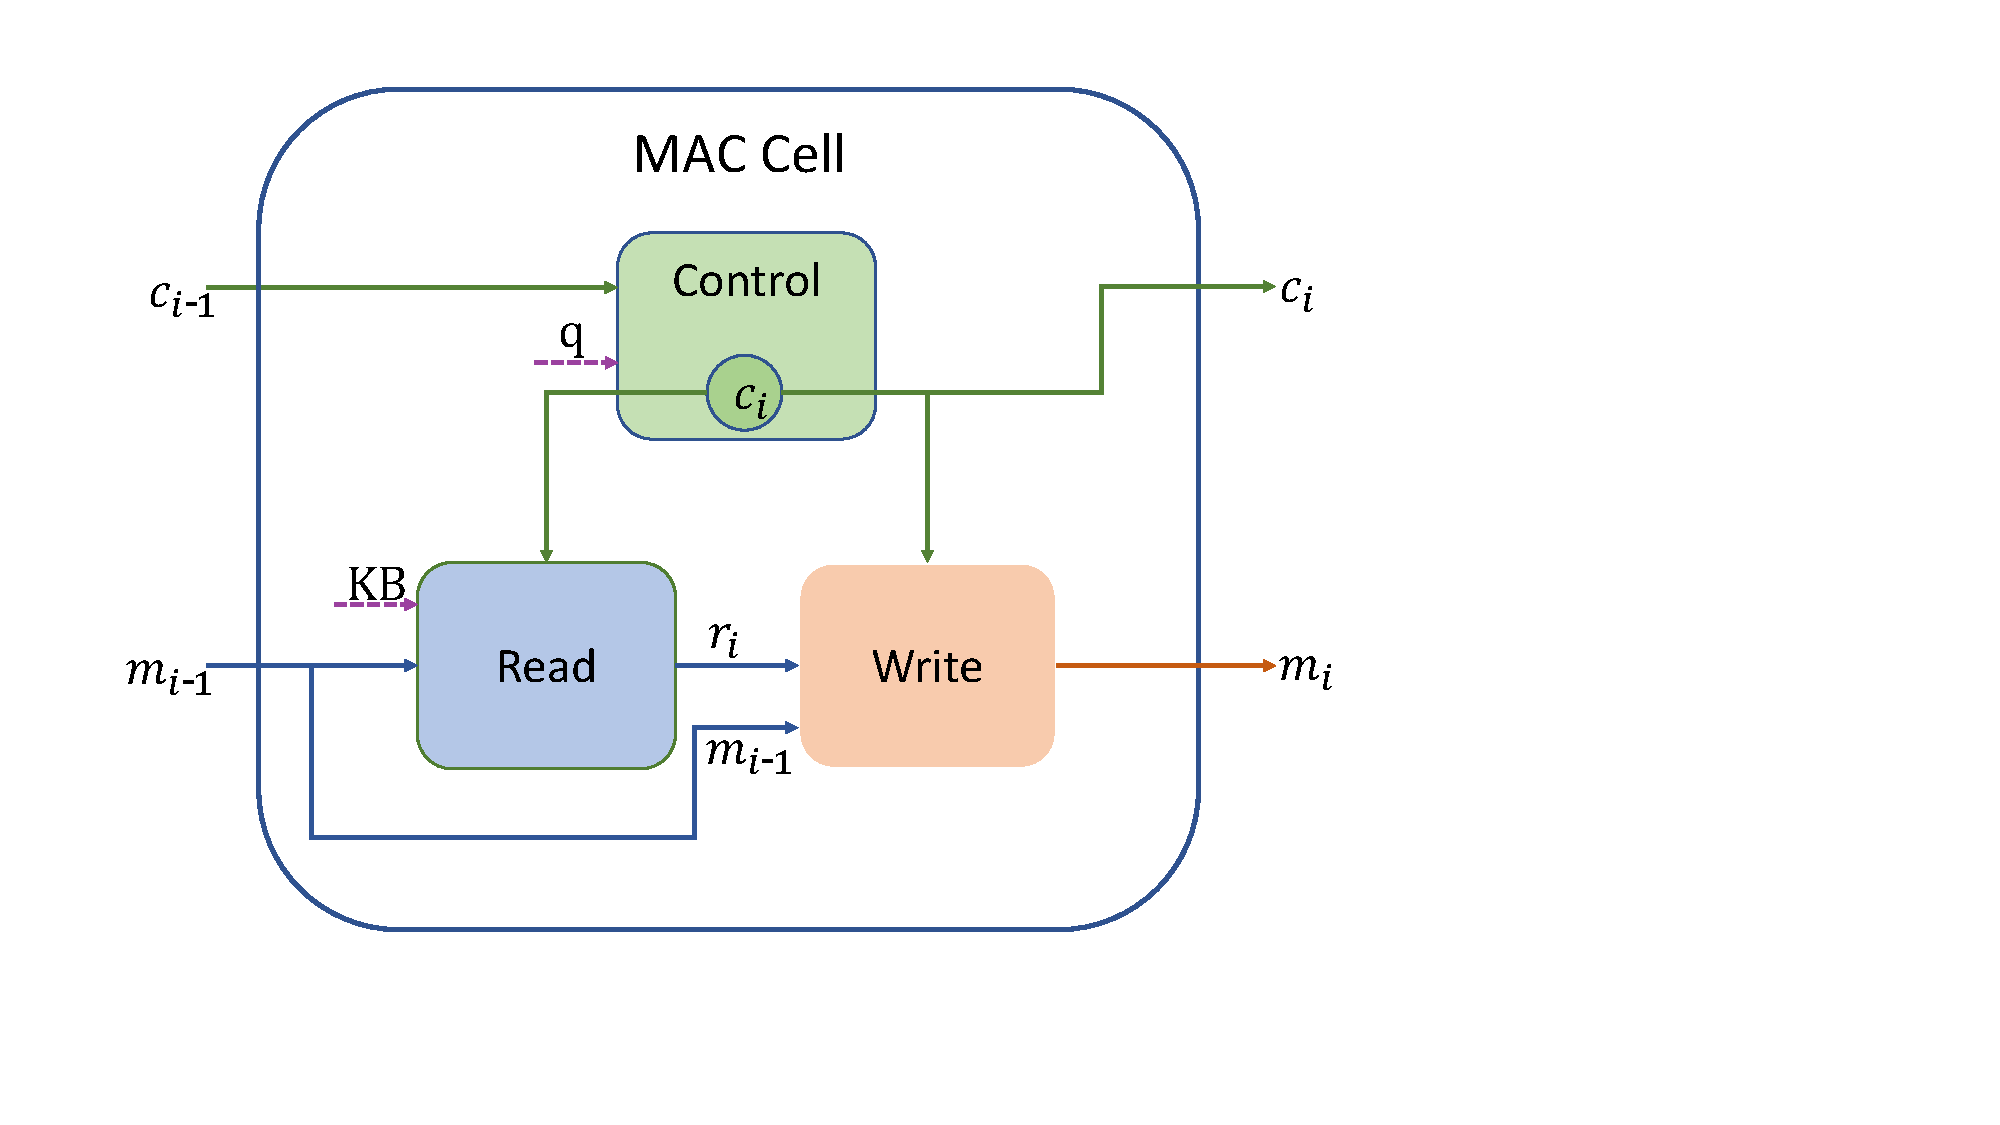
\includegraphics[width=0.7\textwidth]{img/mac_cell.pdf}
	\caption{The Mac Cell. The MAC recurrent cell consists of a control unit, read unit, and write unit, that operate over dual control and memory hidden states. }
	\label{fig:mac_cell}
\end{figure}

\textbf{\textit{Description of the input unit:}}

The role of the input unit is to preprocess the raw images and questions. 
The images are passed through a feature extractor (ResNet101 cut after layer \textbf{\textit{con4}} ) pre-trained on ImageNet. The output tensor is a feature map that is finally processed by two trainable CNN layers to obtain the knowledge base \textbf{\textit{K}}, the final image representation.

The question first go through a word embedding method and then a bidirectional LSTM.
The question preprocessing leads to two different outputs:

\begin{description}
	\item[$\bullet$] The question representation \textbf{\textit{q}} which is the concatenation of the final hidden states from the backward and forward LSTM passes
	\item[$\bullet$] The contextual words \textbf{\textit{cw}} : a series of output states \textbf{\textit{cw1}}, . . . , \textbf{\textit{cwS}} that represent each word in the context of the question
\end{description}



\textbf{\textit{Description of the output unit:}}

The output unit simply process the concatenation of the question representation  \textbf{\textit{q}} and the final memory  \textbf{\textit{mp}} to produce a final answer. For CLEVR it is a 2-layer fully-connected softmax classifier.




